\documentclass[11pt,a4paper]{report}
\usepackage[margin=1in]{geometry}
\usepackage[T1]{fontenc}
\usepackage{lmodern}
\usepackage{hyperref}
\usepackage{booktabs}
\usepackage{longtable}
\usepackage{listings}
\usepackage{xcolor}
\usepackage{tikz}
\usetikzlibrary{shapes,arrows.meta,positioning}

\hypersetup{colorlinks=true,linkcolor=blue,urlcolor=blue}
\lstdefinestyle{bash}{
  basicstyle=\ttfamily\small,
  breaklines=true,
  frame=single,
  backgroundcolor=\color{gray!8}
}

\title{CXR Vault Lab Manual\\
\large SW.17 --- dev secrets + full wiring guide}
\author{CXR Ops Lab --- \texttt{cxr-ops-lab}}
\date{2026-05-31}

\begin{document}
\maketitle
\begin{abstract}
\textbf{SW.17}: HashiCorp Vault dev mode (\textbf{:8200}) stores CXR-shaped secrets at
\texttt{secret/cxr/*}. This manual documents \textbf{exactly how it is wired} ---
Compose $\rightarrow$ seed script $\rightarrow$ KV $\rightarrow$ UI --- and where it would
attach to Claim Studio / K8 in a future phase (not live today).
\end{abstract}
\tableofcontents
\newpage

\chapter{How this lab is wired (step by step)}

\section{The chain (what runs when you type the commands)}

\begin{enumerate}
  \item \textbf{You run} \texttt{./scripts/20-vault-up.sh}
  \item Script calls \texttt{docker compose -f compose.vault.yaml up -d}
  \item \textbf{compose.vault.yaml} starts container \texttt{cxr-ops-lab-vault-1}:
    \begin{itemize}
      \item Image \texttt{hashicorp/vault:1.17}, port \textbf{8200:8200}
      \item Dev mode: in-memory store, auto-unsealed
      \item Root token fixed: \texttt{cxr-bootcamp-root} via \texttt{VAULT\_DEV\_ROOT\_TOKEN\_ID}
    \end{itemize}
  \item \textbf{You run} \texttt{./scripts/20-vault-smoke.sh}:
    \begin{itemize}
      \item \texttt{curl :8200/v1/sys/health} --- Vault is up
      \item Calls \texttt{lab/vault/seed-cxr-secrets.sh}
    \end{itemize}
  \item \textbf{seed-cxr-secrets.sh} \texttt{docker exec}s into the Vault container:
    \begin{itemize}
      \item \texttt{vault secrets enable -path=secret kv-v2} (KV version 2 engine)
      \item \texttt{vault kv put secret/cxr/analyzer ...} (and otel, datastores)
    \end{itemize}
  \item \textbf{You open} \texttt{http://localhost:8200}, login with token \texttt{cxr-bootcamp-root}
  \item \textbf{UI path:} Secrets $\rightarrow$ \texttt{secret/} $\rightarrow$ \texttt{cxr/} $\rightarrow$ \texttt{analyzer}
\end{enumerate}

\section{Wiring diagram}

\begin{center}
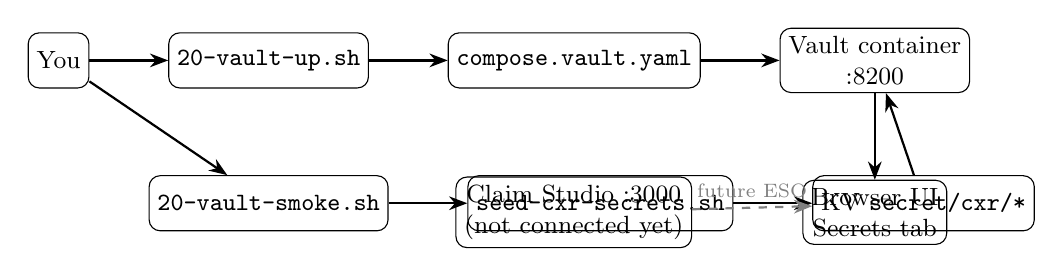
\begin{tikzpicture}[
  node distance=0.55cm and 0.4cm,
  box/.style={draw, rounded corners, minimum height=0.7cm, align=center, font=\small, inner sep=3pt},
  arr/.style={-{Stealth}, thick},
  dashedarr/.style={-{Stealth}, thick, dashed, gray}
]
  \node[box] (you) {You};
  \node[box, right=1cm of you] (up) {\texttt{20-vault-up.sh}};
  \node[box, right=1cm of up] (compose) {\texttt{compose.vault.yaml}};
  \node[box, right=1cm of compose] (vault) {Vault container\\:8200};
  \node[box, below=1.1cm of up] (smoke) {\texttt{20-vault-smoke.sh}};
  \node[box, right=1cm of smoke] (seed) {\texttt{seed-cxr-secrets.sh}};
  \node[box, right=1cm of seed] (kv) {KV \texttt{secret/cxr/*}};
  \node[box, below=1.1cm of vault] (ui) {Browser UI\\Secrets tab};
  \node[box, left=1.4cm of ui] (cxr) {Claim Studio :3000\\(not connected yet)};

  \draw[arr] (you) -- (up);
  \draw[arr] (up) -- (compose);
  \draw[arr] (compose) -- (vault);
  \draw[arr] (you) -- (smoke);
  \draw[arr] (smoke) -- (seed);
  \draw[arr] (seed) -- (kv);
  \draw[arr] (kv) -- (vault);
  \draw[arr] (vault) -- (ui);
  \draw[dashedarr] (cxr) -- node[above,font=\scriptsize]{future ESO} (kv);
\end{tikzpicture}
\end{center}

\chapter{What is wired vs not wired}

\begin{center}
\begin{tabular}{p{4.5cm}p{4cm}p{4.5cm}}
\toprule
\textbf{Layer} & \textbf{Status today} & \textbf{Future (sketch)} \\
\midrule
Vault container :8200 & \checkmark\, Running via Compose & Production Vault cluster \\
\texttt{secret/cxr/*} keys & \checkmark\, Seeded by script & Same paths, stricter ACLs \\
Claim Studio :3000 & \textbf{Not connected} & \texttt{analyze/route.ts} reads env \\
Rehearsal :8251 & \textbf{Not connected} & Same \\
K8 pod :8081 & \textbf{Not connected} & External Secrets $\rightarrow$ Vault $\rightarrow$ pod env \\
\bottomrule
\end{tabular}
\end{center}

\textbf{Today} Claim Studio still gets \texttt{CXR\_ANALYZER\_SCRIPT} from \texttt{.env.local} / compose env.
\textbf{This lab} proves the \emph{secret store} and \emph{path naming} match CXR env inventory (\texttt{lab/vault/cxr-secret-map.json}).

\chapter{Secret map (env $\rightarrow$ Vault path)}

\begin{center}
\begin{tabular}{lll}
\toprule
Vault path & Key & CXR use \\
\midrule
\texttt{secret/cxr/analyzer} & \texttt{CXR\_ANALYZER\_SCRIPT} & Python path for analyze \\
 & \texttt{CXR\_JUDGE\_SCRIPT} & Judge script path \\
\texttt{secret/cxr/otel} & \texttt{OTEL\_*} & SW.11 trace export \\
\texttt{secret/cxr/datastores} & \texttt{QDRANT\_URL} & Vector DB \\
 & \texttt{DATABASE\_URL} & SQL (placeholder) \\
\bottomrule
\end{tabular}
\end{center}

\chapter{UI navigation (after token login)}

\begin{itemize}
  \item \textbf{Ignore for bootcamp:} Dashboard widgets, Access, Policies, Agents
  \item \textbf{Go to:} Secrets $\rightarrow$ engine \texttt{secret/} $\rightarrow$ folder \texttt{cxr/}
  \item \textbf{Golden path:} open \texttt{analyzer} --- confirm \texttt{/analyzers/analyze\_sample.py}
  \item If \texttt{cxr/} is empty: re-run \texttt{./scripts/20-vault-smoke.sh}
\end{itemize}

\chapter{Files in the repo}

\begin{longtable}{@{}p{5.2cm}p{7.8cm}@{}}
\toprule
File & Role in the wiring \\
\midrule
\endhead
\texttt{compose.vault.yaml} & Defines Vault service, port, dev token \\
\texttt{scripts/20-vault-up.sh} & Wrapper: \texttt{compose up -d} \\
\texttt{scripts/20-vault-smoke.sh} & Health + calls seed + reads golden secret \\
\texttt{lab/vault/seed-cxr-secrets.sh} & \texttt{docker exec vault kv put ...} \\
\texttt{lab/vault/cxr-secret-map.json} & Documentation of paths (source of truth for names) \\
\texttt{evidence/SW17-vault-verify-2026-05-31.md} & Checklist \\
\bottomrule
\end{longtable}

\chapter{Hypothetical K8 wiring (not deployed)}

\begin{lstlisting}[style=bash]
# Future sketch only:
# 1. External Secrets Operator installed on kind cluster
# 2. ExternalSecret CR references secret/cxr/analyzer
# 3. Helm chart cxr-ui deployment envFrom -> synced K8 Secret
# 4. Pod at :8081 gets CXR_ANALYZER_SCRIPT without git/env files
\end{lstlisting}

\chapter{Live adjustments}

\begin{itemize}
  \item \textbf{Dev token in compose} --- never use \texttt{cxr-bootcamp-root} in production.
  \item \textbf{KV enable idempotent} --- seed script ignores ``already enabled''.
  \item \textbf{Smoke retry} --- Vault needs a few seconds after \texttt{up}; smoke waits on health.
  \item \textbf{Token login only} --- no username/password in dev mode.
\end{itemize}

\chapter{Procedure}

\begin{lstlisting}[style=bash]
cd cxr-ops-lab
./scripts/20-vault-up.sh
./scripts/20-vault-smoke.sh
# Browser: http://localhost:8200  Token: cxr-bootcamp-root
# Secrets -> secret/cxr/analyzer
\end{lstlisting}

\chapter{Stop}

\begin{lstlisting}[style=bash]
docker compose -f compose.vault.yaml down
\end{lstlisting}

\end{document}
